
\begin{wraptable}{r}{0.29\textwidth}
\vspace{-1.0em}
\centering
\footnotesize
\setlength{\tabcolsep}{5pt}
\renewcommand{\arraystretch}{1.1}
\begin{tabular}{lr}
\toprule
\textbf{Component} & \textbf{Count} \\
\midrule
Semantic groups & 1,400 \\
Domains & 13 \\
\midrule
Anchors/group & 1 \\
SP/group & 20 \\
Soft SC/group & 10 \\
Hard SC/group & 10 \\
\midrule
Total sentences & 57,400 \\
\bottomrule
\end{tabular}
\caption{Dataset composition. Each of the 1,400 semantic groups contains one anchor, 20 SP, 10 soft SC, and 10 hard SC variants.}
\label{tab:dataset_category}
\vspace{-4.0em}
\end{wraptable}

We evaluate the proposed geometric framework through a series of analyses that examine the emergence, structure, and functional role of invariant features across models and layers. Core experiments focus on dataset and model setup, invariant zone localization, geometric validation, causal intervention, and attribution, while extended ablations and additional analyses are deferred to the appendix for completeness. 

\subsection{Evaluation Setup}
\label{sec:eval_setup}

\textbf{Dataset Construction.}
We construct a dataset of 1,400 semantic groups comprising 57,400 sentences across 13 domains (Table~\ref{tab:dataset_category}), covering diverse topics and linguistic contexts to investigate semantic invariance under controlled SP and SC perturbations.
Each group defines a local semantic neighborhood centered on an anchor input. SP variants preserve the underlying meaning while varying lexical form, grammatical structure, and writing style, including formal/casual and question/statement reformulations. Soft SC variants modify an attribute or semantic slot while retaining the original topic, whereas hard SC variants introduce domain- or topic-level semantic changes. For example, given the anchor ``What is the official language of France?'', an SP variant is ``Which language holds official status in France?'', a soft SC variant is ``What is the national currency of France?'', and a hard SC variant is ``What is the longest river in South America?''. Each SC example includes edit-type and source/target-domain metadata, enabling perturbation-specific analysis. Additional construction details and examples are provided in Appendix~\ref{app:expanded_data}.

\begin{wraptable}{r}{0.375\textwidth}
\vspace{-1.0em}
\centering
\footnotesize
\setlength{\tabcolsep}{4pt}
\renewcommand{\arraystretch}{1.1}
\begin{tabular}{llc}
\toprule
\textbf{Model} & \textbf{Family} & \textbf{Params} \\
\midrule
Mistral-Instruct-v0.3 & Mistral  & 7B \\
Llama-3-Instruct      & Llama    & 8B \\
Gemma-IT              & Gemma    & 7B \\
Qwen2.5-Instruct      & Qwen     & 7B \\
GLM-4-Chat            & GLM      & 9B \\
DeepSeek-MoE-Chat     & DeepSeek & 16B \\
InternLM2-Chat        & InternLM & 7B \\
Phi-4-Mini            & Phi      & 4B \\
Falcon3-Instruct      & Falcon   & 7B \\
\bottomrule
\end{tabular}
\caption{Language models used for evaluation, spanning diverse families, scales, and training paradigms.}
\label{tab:models}
\vspace{-1.5em}
\end{wraptable}

To prevent data leakage, each of the 1,400 semantic groups is divided into disjoint discovery and validation subsets, each containing 10 SP and 10 SC variants (5 soft and 5 hard). The discovery subset is used exclusively for invariant subspace identification and layer selection through generalized eigenvalue analysis, while the held-out validation subset is used for downstream evaluation, including tangent-direction validation, representation intervention, projection analysis, and model attribution. This design preserves the local nature of our framework: each group defines an anchor-centered semantic neighborhood with its own invariant subspace. The consistent results across groups support the existence of repeatable local geometric structure rather than a universal invariant projection.

\textbf{Models Analyzed.}
We evaluate nine transformer-based language models listed in Table~\ref{tab:models}, spanning diverse architectural families, parameter scales (4B–16B), and training paradigms. The suite includes models trained under different objectives and pipelines, including instruction tuning, chat alignment, and mixture-of-experts architectures. This diversity allows us to assess whether invariant structure is a consistent property of representation geometry across model families, rather than an artifact of a specific architecture, scale, or training procedure.


\subsection{Localization of Invariant Feature Zones}
\label{sec: localize}

\begin{wrapfigure}{r}{0.4\textwidth}
    \vspace{-1.0em}
    \centering
    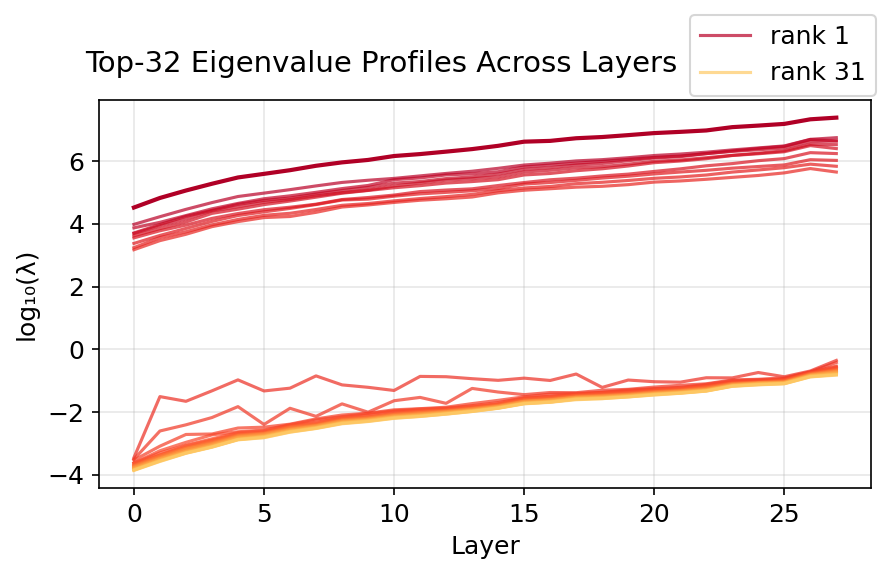
\includegraphics[width=1.0\linewidth]{figures/profiles_einstein.png}
    \vspace{-2.0em}
    \caption{Per-layer eigenvalue profiles for $k=32$ invariant directions (log scale). Each line denotes an eigenvector rank. Eigenvalues increase with depth, and higher-ranked directions remain dominant, indicating a stable and ordered decomposition of invariant signal across layers.}
    \label{fig:eigenvalue_profiles}
    \vspace{-1.0em}
\end{wrapfigure}

We investigate where invariant structure emerges across model depth by analyzing the layer-wise generalized eigenvalue spectrum defined in Section~\ref{sec: find}. The goal is to identify layers in which semantic-changing variation is maximally separated from semantic-preserving variation, corresponding to the emergence of invariant feature zones. 
Since invariant zones are locally defined for each semantic group and model pair, the following analysis presents one representative example from Llama, illustrating how such zones emerge across depth within a specific local semantic neighborhood. 
% \textbf{Experimental Setup.}
For each layer $\ell$, we compute the generalized eigenvalues $\{\lambda_i^{(\ell)}\}_{i=1}^k$ from Eq.~\ref{eq: cross_eigen}, which quantify the ratio between semantic-changing and semantic-preserving variation along each direction. Large eigenvalues indicate directions that are stable under paraphrasing but responsive to semantic change, and therefore correspond to invariant features. We analyze the distribution of the top-$k$ eigenvalues across layers to characterize how invariant structure evolves with depth.


\textbf{Invariant structure becomes more pronounced in mid-to-late layers.} 
Figure~\ref{fig:eigenvalue_profiles} shows the per-layer eigenvalue profiles on a log scale. The leading eigenvalues generally increase with depth, indicating stronger separation between semantic-changing and semantic-preserving variation. However, invariant zones are selected using eigenvalues normalized by the total positive eigenvalue mass within each layer, rather than raw magnitudes alone, reducing bias toward deeper layers. The relative magnitudes of the leading eigenvalues reveal a small set of dominant semantic-sensitive directions, with the strongest separation emerging in mid-to-late layers. This observation is consistent with the local geometric hypothesis in Section~\ref{sec: define}, suggesting that semantic invariance is concentrated in specific depth regions rather than uniformly distributed across layers. These layers are subsequently used to define invariant zones.



\subsection{Tangent-Direction Validation of Invariant Geometry}
\label{sec: tangetD}

We empirically validate the geometric decomposition introduced in Section~\ref{sec: find} by testing whether paraphrase-induced variation concentrates in the nuisance subspace, while semantic displacement lies predominantly outside it. This experiment directly evaluates the geometric structure discovered via contrastive sensitivity decomposition. 

\begin{wraptable}{r}{0.35\textwidth}
\vspace{-1.0em}
\centering
\footnotesize
\setlength{\tabcolsep}{4pt}
\renewcommand{\arraystretch}{1.2}
\begin{tabular}{c|ccc}
\hline
Model 
& G1 
& G4 
& G6 \\
\hline

Mistral 
& 0.0189 & 0.0213 & 0.0198 \\

Llama3 
& 0.0127 & 0.0141 & 0.0135 \\

Qwen2.5
& 0.0158 & 0.0172 & 0.0164 \\

Gemma
& 0.0169 & 0.0184 & 0.0176 \\

Phi4-mini
& 0.0215 & 0.0231 & 0.0223 \\

GLM4
& 0.0112 & 0.0126 & 0.0119 \\

DeepSeek
& 0.0105 & 0.0118 & 0.0112 \\

InternLM2
& 0.0121 & 0.0134 & 0.0128 \\

Falcon3
& 0.0116 & 0.0129 & 0.0123 \\

\hline
\end{tabular}
\caption{Nuisance projection energy $E_{\mathrm{nuis}}$ across models and groups. Low values indicate that semantic displacement lies largely outside the dominant nuisance-sensitive directions.}
\label{tab:energy}
\vspace{-2.0em}
\end{wraptable}

% \textbf{Experimental Setup.}
Let the nuisance component at layer $\ell$ be defined as the Euclidean orthogonal complement of the invariant subspace. Given $U_\ell^{\mathrm{inv}} \in \mathbb{R}^{d \times k}$, the nuisance component of a representation is obtained via the projection operator $(I - U_\ell^{\mathrm{inv}} U_\ell^{\mathrm{inv}\top})$. We do not explicitly construct a nuisance basis, as lower-ranked generalized eigenvectors are not guaranteed to form a stable or Euclidean-orthogonal complement in high-dimensional settings. 
For each semantic group $g=\{x_1,\ldots,x_{n_g}\}$, we compute latent representations $z_i=\Phi_\ell(x_i)$ and define the group centroid $\bar{z}_g=\frac{1}{n_g}\sum_{i=1}^{n_g}z_i$. 
For two semantic groups $g$ and $h$, we define the semantic displacement
\(
\Delta_{gh} = \bar z_g - \bar z_h.
\)
We then evaluate how much of this displacement lies within the nuisance subspace using the projection energy
\(
E_{\mathrm{nuis}} =
\left\|(I - U_\ell^{\mathrm{inv}} U_\ell^{\mathrm{inv}\top}) \, \Delta_{gh}\right\|_2^2  / 
\|\Delta_{gh}\|_2^2.
\) 
Under the local geometric hypothesis, semantic-preserving variations span the nuisance subspace, while semantic differences lie in complementary directions. In this case, the projection operator $(I-U^{\mathrm{inv}}_\ell U^{\mathrm{inv}\top}_\ell)$ removes the semantic component of $\Delta_{gh}$, leaving little residual energy. Consequently, the projected vector $(I-U^{\mathrm{inv}}_\ell U^{\mathrm{inv}\top}_\ell)\Delta_{gh}$ has small norm, leading to $E_{\mathrm{nuis}} \approx 0$. 
Geometrically, $E_{\mathrm{nuis}}$ measures the fraction of semantic displacement energy aligned with nuisance directions. When this value approaches zero, it implies that $\Delta_{gh}$ is nearly orthogonal to the nuisance subspace, and therefore lies primarily in the complementary semantic subspace. This behavior directly reflects the tangent-space decomposition in Eq.~\ref{eq: tan_decompose}, where semantic and nuisance variations occupy distinct, approximately orthogonal directions in the local representation geometry. 
Additional implementation details are provided in Appendix~\ref{appendix: implementation}.

\textbf{Semantic displacement lies predominantly outside the nuisance subspace.}
Table~\ref{tab:energy} reports $E_{\mathrm{nuis}}$ across multiple models and semantic groups. We consistently observe low nuisance projection energy ($\approx 0.01$--$0.02$), indicating that semantic displacement is concentrated in the invariant subspace. This pattern is consistent across models and groups, supporting the proposed local geometric separation between semantic and nuisance directions. Additional comparisons with PCA and cPCA baselines are provided in Appendix~\ref{app:projection_comparison}.




\subsection{Ablation Study: Causal Validation via Representation Intervention}
\label{sec:ab_mainpaper}

We evaluate whether the invariant subspace identified in Section~\ref{sec: find} causally encodes semantic content through representation-level interventions. Rather than relying solely on correlational analysis, these experiments directly perturb the invariant component of the representation and measure the resulting change in model outputs under both within-group and between-group conditions. 
% \textbf{Experimental Setup.}
Given the layer-wise decomposition
\(
z = z_{\mathrm{inv}} + z_{\mathrm{nuis}}
\)
obtained from Eq.~\ref{eq: decompose_z_inv}, we construct interventions by replacing the invariant component of an anchor representation while keeping the nuisance component fixed. In practice, interventions are implemented at the token level using the final-token hidden state $h_\ell^{(T)}(x)$, which directly determines next-token prediction in causal language models. We therefore set
\(
z_\ell(x) = h_\ell^{(T)}(x),
\)
so that
\(
h_\ell^{(T)}(x)=h_{\mathrm{inv}}+h_{\mathrm{nuis}}.
\) 
For an anchor hidden state $h^{(a)}$ and donor hidden state $h^{(d)}$, the intervened representation is
\(
h^{\mathrm{int}}
=
h^{(a)}
+
\alpha
\big(
h_{\mathrm{inv}}^{(d)}
-
h_{\mathrm{inv}}^{(a)}
\big),
\)
which is then propagated through the remaining layers. The intervention effect is measured using the KL divergence between the original and intervened next-token distributions,
\(
\mathrm{KL}(\ell)
=
D_{\mathrm{KL}}
\!\left(
p_{\mathrm{base}}
\,\|\,
p_{\mathrm{int}}
\right).
\) 

\begin{wraptable}{r}{0.45\textwidth}
\vspace{+0.25em}
\centering
\footnotesize
\setlength{\tabcolsep}{3pt}
\renewcommand{\arraystretch}{1.1}
\begin{tabular}{lccc}
\toprule
\textbf{Model} 
& \textbf{Between} 
& \textbf{Within-SP} 
& \textbf{Within-SC} \\
& KL$\uparrow$ & KL$\downarrow$ & KL$\uparrow$ \\
\midrule
Mistral-7B       & 0.974 & 0.036 & 0.341 \\
Llama-3-8B       & 0.986 & 0.040 & 0.360 \\
Gemma-7B         & 0.979 & 0.042 & 0.382 \\
Qwen2.5-7B       & 0.984 & 0.047 & 0.401 \\
GLM-4-9B         & 0.983 & 0.034 & 0.337 \\
DeepSeek-MoE     & 0.985 & 0.052 & 0.427 \\
InternLM2-7B     & 0.984 & 0.039 & 0.354 \\
Phi-4-mini       & 0.981 & 0.045 & 0.391 \\
Falcon3-7B       & 0.986 & 0.049 & 0.418 \\
\bottomrule
\end{tabular}
\caption{Invariant-component intervention results. Between-group swaps use donors from a different semantic group; within-group swaps use SP or SC donors from the same group. Low within-SP KL and high within-SC/between-group KL indicate semantic selectivity of the invariant subspace.}
\label{tab:inv_intervention_combined}
\vspace{-1.5em}
\end{wraptable}

We consider three intervention settings. In the within-group SP setting, the donor is a paraphrase from the same semantic group. In the within-group SC setting, the donor is semantically different but remains within the same semantic neighborhood. In the between-group setting, the donor is drawn from a completely different semantic group. Under the geometric hypothesis, SP interventions should produce minimal output change, while SC and between-group interventions should induce substantially larger shifts due to semantic inconsistency. 

\textbf{Invariant-component interventions produce substantially larger output changes under semantic-changing than semantic-preserving perturbations.}
Table~\ref{tab:inv_intervention_combined} summarizes KL divergence across all three intervention settings. Within-group SP interventions consistently produce near-zero KL divergence across models, indicating that the discovered invariant representation remains stable under paraphrastic variation. In contrast, within-group SC interventions yield substantially larger KL divergence, indicating that the invariant subspace is sensitive to semantic change even within a locally related semantic region. The effect becomes even stronger in the between-group setting, where invariant-component replacement produces consistently large KL divergence across all models. Together, these results provide evidence consistent with a causal role of the discovered invariant subspace in semantically meaningful model behavior. The separation between invariant- and nuisance-component interventions is further supported by narrow 95\% bootstrap confidence intervals across semantic groups (Appendix~\ref{app:bootstrap}) and remains evident in multi-hop reasoning tasks (Appendix~\ref{app:multihop}).


\subsection{Robust Model Attribution via Invariant Features}

\begin{wraptable}{r}{0.6\textwidth}
\vspace{-1.0em}
\centering
\scriptsize
\setlength{\tabcolsep}{4.5pt}
\renewcommand{\arraystretch}{1.3}
\begin{tabular}{c|ccc|ccc|ccc}
\hline
\multirow{2}{*}{Model} 
& \multicolumn{3}{c|}{Group1}
& \multicolumn{3}{c|}{Group2}
& \multicolumn{3}{c}{Group3} \\

& B & FT & D
& B & FT & D
& B & FT & D \\
\hline

Mistral 
& 93.2 & 91.4 & 89.8 
& 92.7 & 91.0 & 89.4 
& 93.5 & 91.8 & 90.2 \\

Llama3
& 94.1 & 92.5 & 90.9 
& 93.8 & 92.1 & 90.5 
& 94.4 & 92.9 & 91.3 \\

Gemma 
& 92.8 & 90.9 & 89.2 
& 92.3 & 90.5 & 88.8 
& 93.0 & 91.2 & 89.6 \\

Qwen2.5
& 93.6 & 91.8 & 90.1 
& 93.1 & 91.3 & 89.7 
& 93.9 & 92.0 & 90.5 \\

Phi4-mini
& 89.6 & 87.8 & 86.1 
& 89.2 & 87.4 & 85.8 
& 90.1 & 88.2 & 86.5 \\

GLM4
& 95.2 & 93.6 & 91.9
& 94.8 & 93.1 & 91.5
& 95.6 & 94.0 & 92.3 \\

DeepSeek
& 95.8 & 94.2 & 92.6
& 95.3 & 93.7 & 92.0
& 96.1 & 94.5 & 92.9 \\

InternLM2
& 94.9 & 93.3 & 91.7
& 94.5 & 92.9 & 91.3
& 95.2 & 93.6 & 91.9 \\

Falcon3
& 95.5 & 93.9 & 92.2
& 95.0 & 93.4 & 91.8
& 95.8 & 94.2 & 92.5 \\

\hline
\end{tabular}
\caption{Attribution accuracy (\%) across Base (B), Fine-tuned (FT), and Distilled (D) variants for three representative groups. Performance remains high and stable under model adaptation.}
\label{tab:model_wise_attribution}
\vspace{-1.25em}
\end{wraptable}

For each model $m \in \mathcal{F}$, attribution is performed by comparing the invariant representation of a test model to reference model signatures using the method defined in Section~\ref{sec: attribution_app}. 
To assess robustness, we consider three variants of each model: the original base pretrained model (B), a fine-tuned version (FT), and a distilled version (D). Fine-tuned models are obtained via instruction tuning on downstream tasks, while distilled models are trained to approximate teacher outputs with reduced capacity. Importantly, prototype invariant zones are computed from the original models and reused without modification for testing the FT and Dist variants. This protocol isolates whether invariant features reflect intrinsic representation geometry rather than training-specific adaptations. Additional implementation details for fine-tuned and distilled model variants, checkpoint construction, layer-selection protocol, and attribution evaluation are provided in Appendix~\ref{app:model_variants}.

\textbf{Invariant representations enable accurate model attribution and remain robust under fine-tuning and distillation.}
Table~\ref{tab:model_wise_attribution} reports attribution accuracy across models and variants. We observe consistently high accuracy for original base models (typically above $92\%$), indicating that invariant zone representations capture strong model-specific signatures. Attribution performance remains high under both fine-tuning and distillation, with only modest degradation (approximately $2$--$4\%$ across models). These results suggest that the discovered invariant features capture model-specific geometric structure that persists under model adaptation, despite changes in task behavior and model parameterization. 
% Additional attribution comparisons against PCA and cPCA projection baselines are provided in Appendix~\ref{app:attribution_baseline}.


\begin{wraptable}{r}{0.35\textwidth}
\vspace{+0.5em}
\centering
\scriptsize
\setlength{\tabcolsep}{5pt}
\renewcommand{\arraystretch}{1.2}
\begin{tabular}{lccc}
\toprule
\textbf{Variant} & \textbf{PCA} & \textbf{cPCA} & \textbf{Ours} \\
\midrule
Base & 86.08 & 89.33 & \textbf{95.45} \\
Fine-tuned & 83.98 & 87.53 & \textbf{94.20} \\
Distilled & 81.25 & 84.65 & \textbf{92.25} \\
\bottomrule
\end{tabular}
\caption{Zero-shot attribution accuracy (\%) averaged over four models (Llama, Mistral, Qwen2.5, and Gemma) with matched subspace dimensionality. Unlike Table~\ref{tab:model_wise_attribution}, these results are aggregated over the full evaluation set. Full results are in Appendix~\ref{app:attribution_baseline}.}
\label{tab:attribution_baseline_main}
\vspace{-1.25em}
\end{wraptable}


\textbf{Contrastive invariant decomposition outperforms variance-based and contrastive baselines in model attribution.}
To determine whether attribution performance arises from the proposed invariant geometry rather than generic representation structure, we compare our method against PCA and contrastive PCA (cPCA) using matched subspace dimensionality. PCA selects directions of dominant representation variance, while cPCA identifies directions maximizing the contrast $S_{\mathrm{SC}}-\alpha S_{\mathrm{SP}}$. In contrast, our generalized eigenvalue formulation identifies directions with high SC sensitivity relative to SP variation. Table~\ref{tab:attribution_baseline_main} summarizes accuracy averaged across four model families. Our method consistently outperforms both baselines under all adaptation settings, improving over cPCA by 6.13, 6.68, and 7.60 percentage points for base, fine-tuned, and distilled models, respectively. These results indicate that normalizing semantic-changing variation relative to semantic-preserving sensitivity provides more discriminative model signatures than variance maximization or additive covariance contrast alone. Full model-wise comparisons and experimental details are provided in Appendix~\ref{app:attribution_baseline}.



